%!TeX root = Thesis_LP.tex
\chapter{La sismique comme outil de surveillance du \texorpdfstring{\ce{CO2}}{CO2}}
\label{sc:sismique}
Cette section décrit brièvement les bases théoriques et les démarches méthodologiques nécessaires pour répondre au premier objectif de l’étude. La \cref{sc:theorie_sismique} présente la base théorique de la propagation des ondes acoustiques dans les milieux poreux. Les détails de la méthodologie utilisée se retrouvent dans l’article I faisant partie de cette thèse. Afin d'éviter la redondance, les \cref{sc:laboratoire,,sc:model} présentent un survol sur la méthodologie utilisée pour les mesures de laboratoires et pour la modélisation sismique de l'injection du \ce{CO2} et une discussion sur les résultats. 
% \section{La sismique comme outil de surveillance du \texorpdfstring{\ce{CO2}}{CO2}}
% \label{sc:sismique}
\section{Concepts théoriques de base}
\label{sc:theorie_sismique}
\subsection{Les milieux élastiques}
 On appelle onde sismique toute onde mécanique qui traverse un milieu géologique. Dans l'analyse des données sismiques, on utilise souvent l'approximation d'élasticité, c'est à dire que les particules reviennent à leur place après le déplacement imposé par l'onde mécanique.\\
La théorie de l'élasticité part du principe que si un solide est soumis à des contraintes, il se déforme et lorsque la contrainte est retiré il reprend sa forme initiale. En sismique, on impose a priori que forces et déformations soient minimes et donc que les relations entre forces et déformations soient linéaires, ce qui permet de représenter le milieu comme parfaitement élastique où toute l'énergie est conservé \citep{Sheriff1995}. Il existe deux types de contraintes, définis par l’orientation selon lesquelles la force est exercée. Si la force est appliquée perpendiculairement à la surface, on parle de contrainte normale, si elle est appliquée de façon tangentielle, on parle de contrainte de cisaillement. Le comportement mécanique d’un milieu élastique, anisotrope et linéaire peut être décrit par la loi de Hooke généralisé:
\begin{equation}
\sigma_{ij} = C_{ijkl}*\epsilon_{kl} \qquad i,j,k,l = 1,2,3
\label{eq:hooke}
\end{equation}
où $\sigma$ représente la contrainte, $C$ est le tenseur de rigidité de la matrice et $\epsilon$ est la déformation.
La contrainte et la déformation peuvent être rapresentée par des matrices $3 \times 3$ (9 composantes) qui représentent la tridimensionnalité d’un volume. Le comportement du materiel peut donc être modélisé par un tenseur de rigidité de 81 composantes ($3 \times 3 \times 3 \times 3$) qui sont réduites à 21 grâce à la symétrie entre la contrainte et la déformation. Il s’agit du numéro maximal de composantes qu’un milieu homogène linéaire peut avoir. Un milieu isotrope, qui présente la symétrie maximale, est caractérisé par deux composantes indépendantes, tandis que les milieux avec une symétrie triclinique sont représentés par tous les 21 composantes.\\
C’est une pratique courante d’utiliser la notation de Voigt pour représenter les contraintes, les déformations et les tenseurs de rigidité. Avec cette notation, les contraintes et les déformations deviennent des vecteurs de six éléments plutôt que des matrices carrées de 9 éléments. Avec la notation de Voigt, les 4 indices du tenseur de rigidité sont réduits à deux, en utilisant la convention suivante:
$$\begin{matrix}
ij(kl) & I(J)\\
 11 & 1 \\
 22 & 2 \\
 33 & 3 \\
 23, 32 & 4 \\
 13, 31 & 5 \\
 12, 21 & 6 \\
\end{matrix}$$
En utilisant la notation de Voigt, on peut écrire l’\cref{eq:hooke} sous cette forme:
\[ 
    \begin{bmatrix}
        \sigma_{1} \\
        \sigma_{2} \\ 
        \sigma_{3} \\
        \sigma_{4} \\
        \sigma_{5} \\
        \sigma_{6} \\
    \end{bmatrix}
    =
    \begin{bmatrix}
        C_{11} & C_{12} & C_{13} & C_{14} & C_{15} & C_{16} \\
        C_{12} & C_{22} & C_{23} & C_{24} & C_{25} & C_{26} \\
        C_{13} & C_{23} & C_{33} & C_{34} & C_{35} & C_{36} \\
        C_{14} & C_{24} & C_{34} & C_{44} & C_{45} & C_{46} \\
        C_{15} & C_{25} & C_{35} & C_{45} & C_{55} & C_{56} \\
        C_{16} & C_{26} & C_{36} & C_{46} & C_{56} & C_{66} \\
    \end{bmatrix}
    \begin{bmatrix}
        \epsilon_{1} \\
        \epsilon_{2} \\ 
        \epsilon_{3} \\
        \epsilon_{4} \\
        \epsilon_{5} \\
        \epsilon_{6} \\
    \end{bmatrix}
.\]
Dans le cas isotrope, la matrice de rigidité s’écrit comme suit:
\[ 
    \begin{bmatrix}
        C_{11} & C_{12} & C_{12} &   0    &   0    &    0   \\
        C_{12} & C_{11} & C_{12} &   0    &   0    &    0   \\
        C_{12} & C_{12} & C_{11} &   0    &   0    &    0   \\
           0   &   0    &   0    & C_{44} &   0    &    0   \\
           0   &   0    &   0    &   0    & C_{44} &    0   \\
           0   &   0    &   0    &   0    &   0    & C_{44} \\
    \end{bmatrix}
, \qquad C_{12} = C_{11} - 2C_{44}
\]
Les relations entre les constantes élastiques $C$  et les paramètres de Lamé $\lambda$ et $\mu$ pour un milieu isotrope sont:
\begin{equation}
C_{11} = \lambda + 2\mu = K + \frac{4}{3}\lambda, \qquad C_{12} = \lambda, \qquad C_{44}= \mu,
\end{equation} 
où $K$ est le \textbf{module d'incompressibilité} et $\lambda$ le \textbf{module de cisaillement} du milieu.
En sismique, la propagation des ondes est généralement donnée en terme de module d'incompressibilité et de cisaillement car ils ont des interprétations physiques claires. Le premier est essentiellement la mesure de la résistance du milieu à une compression uniforme (rigidité). Le module de cisaillement, ou deuxième paramètre de Lamé est une mesure de la résistance du milieu à une déformation de cisaillement. Le premier paramètre de Lamé, $\lambda$, n'a aucune interprétation physique, mais il intervient dans la simplification de la matrice de rigidité. \\
D'autres modules peuvent être utilisés pour décrire un milieu isotrope sous une contrainte uniaxiale. Le \textbf{module de Young} $E$ est le rapport entre la contrainte appliquée et l'allongement relatif. Le \textbf{coefficient de Poisson} est le rapport entre la déformation transversale et axiale. Dans le cas d'une déformation uniaxiale, on peut utiliser le \textbf{module des ondes P} défini comme le rapport entre la contrainte et la déformation axiale. Pour de plus amples détails sur le sujet des milieux élastiques voici quelques références: \citet{Bourbie1986,Carcione2007,Mavko2009} 
\subsection*{La propagation des ondes dans les milieux élastiques}
\label{sc:prop_ondes}
Dans la section précédente, la relation entre contrainte appliquée et déformation a été établie en utilisant la loi de Hooke. Cependant, cette loi ne donne pas la variation du déplacement des points du milieu avec le temps. La propagation d’une onde dans l’espace et dans le temps peut être décrite si le volume du milieu considéré n’est pas en équilibre statique. La deuxième loi du mouvement de Newton indique qu’une force non nulle exercée sur un corps est égale au produit de la masse et de l’accélération du corps. En incluant la loi de Hooke dans l’équation du mouvement et en exprimant la déformation en terme de déplacement, l’équation d’onde à une dimension dans un milieu élastique pour un déplacement $u$ est donnée par:
\begin{equation}
\rho\frac{\partial^2 u}{\partial t^2} = C\nabla^2u,
\label{eq:onde}
\end{equation}
où $u$ est fonction de la position et du temps, $\rho$ est la densité du milieu élastique et $C$ et la constante de rigidité ou module élastique relative au type d'onde pris en considération. La vitesse de l'onde pour le cas le plus général de l'\cref{eq:onde} est:
\begin{equation}
V = \sqrt{\frac{C}{\rho}}
\label{eq:velocity_gen}
\end{equation}
Essentiellement, l’équation d’onde met en relation la dérivée dans le temps avec la dérivée dans l’espace du déplacement par la constante de proportionnalité de $V^2$.\\
Dans un milieu homogène isotrope, il y a 2 types d’ondes principaux qui sont étudiées, les ondes de compression $P$ et les ondes de cisaillement $S$. Pour la vitesse des ondes $P$ et $S$, l'\cref{eq:velocity_gen} devient:
\begin{equation}
V_p = \sqrt{\frac{C_{11}}{\rho}} = \sqrt{\frac{\lambda + 2\mu}{\rho}} = \sqrt{\frac{K+\frac{4}{3}\mu}{\rho}}\quad et
\label{eq:vitesse_p}
\end{equation}
\begin{equation}
V_s = \sqrt{\frac{C_{44}}{\rho}} = \sqrt{\frac{\mu}{\rho}} ,
\label{eq:vitesse_s}
\end{equation}
respectivement. Les fluides ne peuvent pas soutenir les forces de cisaillement, le module de cisaillement de fluides est donc égal à zéro. Seulement les ondes $P$ peuvent voyager dans des liquides dont la vitesse de l’onde est:
\begin{equation}
V_p = \sqrt{\frac{K}{\rho}} .
\label{eq:velocity_pliq}
\end{equation}
La théorie présentée jusqu'ici s'applique à des milieux monophasiques (solides). Pour de plus amples détails sur la propagation des ondes dans ce type de milieu, voici quelques références: \citet{Sheriff1995,Aki1980}.\\

Pour étendre l'étude de la propagation des ondes dans des milieux poreux saturés de fluide, on applique le modèle de Biot \citep{Biot1956a,Biot1956b}. Dans ce modèle, les interactions fluide-structure sont prises en compte à travers trois types de couplage : les couplages massiques, élastiques et visqueux.
\subsection{Les milieux viscoélastiques}
Le comportement viscoélastique est une réponse mécanique, en fonction du temps, d'un milieu à des variations de contrainte appliquée. \citet{Boltzmann1874} a été parmi les premiers scientifiques à introduire le concept de mémoire: pour un point donné d'un milieu, la contrainte appliquée au temps $t$ dépend de la déformation du milieu au temps $t-1$. Différemment d'un milieu purement élastique, où l'énergie utilisée pour déformer le milieu est conservée, dans un milieu viscoélastique, elle est complètement dissipée. N'ayant plus d'énergie pour retourner à l'état initial, un milieu viscoélastique reste donc déformé \citep{Carcione2007}. \\
Le facteur adimensionnel de qualité $Q$ permet de caractériser la dissipation d'un milieu. Par définition, le facteur Q est inversement proportionnel à l’énergie absorbée par le milieu lors d’un cycle d’oscillation de l’onde \citep{Sheriff1995}.  Cette définition revêt la forme
mathématique suivante:
\begin{equation}
Q = \dfrac{2\pi}{\dfrac{\Delta E}{E}}.
\label{eq:facteur_Q}
\end{equation}
Ainsi, plus le matériau est de piètre qualité du point de vue sismique, plus l’énergie de l’onde sismique dissipée ($\Delta E$) est grande, plus le facteur de qualité sera faible \citep{Giroux2001}. Pour un système viscoélastique, il y a une relation directe entre la vitesse de dispersion et le facteur de qualité. 
\subsection{Les milieux poroviscoélastiques}
Le concept de viscoélasticité peut être introduit dans les équations de Biot \citep{Biot1956a,Biot1956b} pour la modélisation des mécanismes d'atténuation liée à l'énergie de déformation (dissipation due à la rigidité) et à l'énergie cinétique (dissipation viscodynamique) \citep{Carcione2007}. \citet{Carcione1998} a modifié les équations de Biot afin d'inclure des mécanismes d'interaction matrice-fluide à travers les fonctions de relaxation viscoélastique. Cette formulation est la plus appropriée pour décrire le phénomène de l'injection du \ce{CO2} dans des grès, car il permet d’inclure les propriétés des fluides dans les équations de propagation des ondes.\\
Les développements mathématiques pour la propagation des ondes dans les milieux viscoélastiques et poroviscoélastiques sont détaillés dans \citet{Bourbie1986} et \citet{Carcione2007}
\subsection{La physique de roches}
La discipline de la physique de roches a comme objectif d'établir des relations entre les propriétés des roches et la réponse physique observée. Dans notre cas, la physique des roches étudie les propriétés physiques qui influencent la propagation des ondes sismiques à travers les roches, à savoir la compressibilité, la rigidité, la porosité, la densité et les fluides interstitiels. Pour établir ces relations, il faut connaître les propriétés élastiques de la matrice et des fluides interstitiels ainsi que les modèles d'interaction entre fluide et roche. \\
Le concept de substitution de fluide se réfère à la modélisation des vitesses des ondes sismiques dans un milieu poreux saturé, à partir de l'information obtenue du milieu poreux sec ou à partir du milieu poreux saturé avec un autre fluide.
\subsubsection{L'équation de Gassmann}
En physique de roches, la relation de Gassmann \citep{Gassmann} est fréquemment utilisée en raison de sa simplicité et applicabilité dans la gamme de fréquences sismiques, autour de \SI{100}{\hertz} \citep{Mavko2009}. Dans sa formulation,  Gassmann, fais plusieurs hypothèses:
\begin{enumerate}
\item La roche est considérée comme homogène et isotrope;
\item Les minéraux constituant la roche ont le même module de rigidité et de cisaillement;
\item Les fluides interstitiels peuvent circuler librement et les pores sont connectés entre eux;
\item Les pores sont complètement saturés;
\item Les fluides interstitiels n'interagissent pas avec les minéraux de la roche;
\item Les fréquences sont suffisamment basses pour que la pression induite dans les pores puisse se rééquilibrer.
\end{enumerate} 
Dans l’équation de Gassmann, le module de la roche saturée $K$ est relié au module de la matrice (roche sèche) $K_{dry}$, le module de la roche solide (minéraux constituant la roche) $K_s$, le module du fluide interstitiel $K_f$ et la porosité de la roche $\phi$ par \citep{Mavko2009}:
\begin{equation}
\dfrac{K}{K_s - K} = \dfrac{K_{dry}}{K_s - K_{dry}} + \dfrac{K_f}{\phi (K_s - K_f)},
\end{equation}
en réarrangeant, on a:
\begin{equation}
K = K_{dry} + \dfrac{\bigg(1 - \dfrac{K_{dry}}{K_s}\bigg)^2}{\dfrac{\phi}{K_f}+\dfrac{1-\phi}{K_s} + \dfrac{K_{dry}}{K_s^2}}.
\label{eq:gasmmann}
\end{equation}
Si le module de la roche sèche $K_{dry}$ n'est pas disponible, le module de la roche saturée  $K$ peut être lié au module de la roche saturée avec un autre fluide $K_2$ selon la relation suivante\citep{Mavko2009}:
\begin{equation}
\dfrac{K}{K_s - K} - \dfrac{K_{f}}{\phi(K_s - K_{f})} = \dfrac{K_2}{K_s - K_2} - \dfrac{K_{f2}}{\phi(K_s - K_{f2})}.
\end{equation}
Dans la formulation de Gassmann, le module de cisaillement est indépendant des fluides qui saturent la roche, car ces derniers sont incapables de soutenir des forces de cisaillement. Donc, le module de cisaillement de la roche saturée est égal au module de cisaillement de la roche sèche:
\begin{equation}
\mu_{sat} = \mu_{dry}
\end{equation}
À partir des résultats de $k$ et $\mu$, les vitesses $V_p$ et $V_s$ correspondantes peuvent être calculées en utilisant les \cref{eq:vitesse_p,,eq:vitesse_s} où la densité de la roche saturée est:
\begin{equation}
\rho_{sat} = (1-\phi)\rho_s + \phi \rho_f.
\end{equation}
 
Avant d'effectuer la substitution de fluide en utilisant l'\cref{eq:gasmmann}, il faut déterminer la porosité ($\phi$), les propriétés des fluides interstitiels ($K_f$, $\rho_f$), le module de la matrice ($K_{dry}$ ainsi que le module des solides ($K_s$) de la roche. Ces quatre composantes peuvent être inférées avec des mesures de laboratoire ou avec l'analyse de diagraphies. Une revue exhaustive sur les méthodes pour les déterminer se trouve dans \citet{Smith2003} et \citet{Mavko2009}.
\subsubsection{La formulation de Biot}
À différence de Gassmann, Biot prédit la dépendance en fréquence des vitesses des ondes dans les milieux saturés. Il a présenté sa théorie pour les basses et les hautes fréquences dans \citet{Biot1956a,Biot1956b}. Pour les basses fréquences, la relation de Biot se réduit à celle de Gassmann. Les mêmes hypothèses que pour Gassmann s'appliquent. De plus, Biot suppose que les fluides interstitiels sont newtoniens. Dans sa formulation, Biot représente la dépendance en fréquence des ondes en incorporant les interactions visqueuses et inertielles entre le fluide interstitiel et la matrice solide de la roche. \\
Pour les hautes fréquences, les fluides interstitiels n'ont pas assez de temps pour se rééquilibrer donnant naissance à des phénomènes d’atténuation et dispersions connus sous le nom d'écoulement de fluide induit par la propagation des ondes, de l'anglais \emph{wave-induced fluid flow} \citep{Muller2010}.\\
Les bases mathématiques de la formulation de Biot sont développées dans les articles originaux \citet{Biot1956a,Biot1956b} ainsi que dans \citet{Bourbie1986}, \citet{Carcione2007} et \citet{Allard2009}. 
\section{Mesures sismiques de laboratoire sous injection de \texorpdfstring{\ce{CO2}}{CO2}}
\label{sc:laboratoire}
La première étape de ma thèse a été de vérifier et de mesurer la relation entre les propriétés physiques et géologiques dans les conditions de pression et température des réservoirs potentiels du Québec. Ces mesures m'ont poussé à aller effectuer un stage de 3 mois dans le laboratoire du professeur Schmitt à l'université d'edmonton.

La méthode de la transmission par impulsion est parmi les méthodes ultrasoniques les plus utilisées en physique de roches \citep{Wyllie1958,Nur1971,Timur1977,Toksz1979,Tosaya1982,Blair1990,Wang1991,Cadoret1995,Adam2006,Verwer2008,Yam2011,Njiekak2013,Schmitt2015} et elle est la seule méthode appliquée à ce jour pour les études en laboratoire du \ce{CO2} sur les ondes élastiques. En comparaison avec d'autres techniques, la transmission par impulsion est relativement simple et facilement applicable. Des variables telles que la pression, la température et la saturation peuvent être manipulées pour étudier leur effet sur la réponse sismique. \\ 
L'approche proposée dans cette étude s'inspire directement de \citet{Schmitt2015} et les réponses sismiques associées aux différentes phases du \ce{CO2} ont été étudiées sur deux échantillons du Covey Hill et du Cairnside complètement saturés en \ce{CO2} avec la méthode de transmission par impulsion. Avec cette méthode, l'échantillon est placé entre la source et un récepteur qui sont généralement des transducteurs piézoélectriques en céramique. Les mesures ont été acquises dans le laboratoire de géophysique de l'université de l'Alberta sous la supervision du professeur Douglas R. Schmitt. La \cref{sc:art_1_ultrasonic_measurements} de l'article I à la \cpageref{sc:art_1_ultrasonic_measurements} décrit la procédure des mesures de laboratoire, de la préparation des échantillons jusqu'aux analyses. Les paragraphes qui suivent donnent un aperçu des étapes principales.
\subsection{Préparation des échantillons}
Deux échantillons cylindriques de \SI{3.7}{\cm} et de \SI{4}{\cm} de longueur ont été préparés pour les analyses. Un aspect très important pour améliorer la transmission du signal et pour minimiser les erreurs de mesure est de s'assurer que les extrémités de l'échantillon soient les plus parallèles possible entre eux. Les échantillons ont été initialement taillés afin de les rendre approximativement parallèles et ensuite ont été polis en utilisant une meuleuse afin que le parallélisme entre les extrémités soit de l'ordre de \SI{\pm0.025}{\mm}. Avant de commencer les mesures, les deux échantillons ont été séchés dans une étuve à \SI{70}{\degreeCelsius} pendant \numrange{24}{36} heures et déposés dans un dessiccateur.\\
L'étape finale de la préparation consiste à sceller l'assemblage avec un tube Tygon\texttrademark{} qui assure l’étanchéité à l'huile hydraulique présente à l’intérieur de la cuve sous pression où les mesures sont effectuées. La \cref{fig:apparatus} de l’article I à la \cpageref{fig:apparatus} montre l'assemblage de l'échantillon avec les transducteurs scellés dans le tube de Tygon\texttrademark{} prêt pour être introduit dans la cuve sous pression (désigné avec la lettre A dans la même figure). Cette figure montre aussi le système de pompage pour régler la pression de confinement et interstitielle. La \cref{sc:experimental_apparatus} de l'article I à la \cpageref{sc:experimental_apparatus} décrit les caractéristiques des différentes parties de l'équipement de mesure utilisé dans le cadre de ma thèse.
\subsection{Procédure expérimentale}
Les échantillons ont été soumis à une série de mesures, y compris des mesures en conditions sèches et différentes conditions de saturation en \ce{CO2}. Avant de décrire les mesures, c’est important de définir les types de pression qui peuvent être appliqués aux échantillons. Comme décrit dans la section précédente, le système des pompes peut contrôler deux types de pressions; la pression appliquée à la superficie de l’échantillon (pression de confinement) et la pression du fluide interstitiel (pression de pore). Ces deux types de pressions sont exercées dans des directions opposées et l’on définit la pression différentielle $P_d$ comme suit:
\begin{equation}
P_d = P_c - P_p,
\end{equation}
où $P_c$ est la pression de confinement qui est généralement plus large de la pression de pore $P_p$. Dans le cas où $P_p$ est plus grande que $P_c$ on a fracturation hydraulique de la roche.\\
Les caractéristiques des mesures effectuées pour les échantillons du Covey Hill et du Cairnside sont résumées dans le \cref{tbl:measures}.
\begin{table}[tb]
    \caption{Type de mesures effectuées sur les échantillons du Covey Hill et du Cairnside.}
    \label{tbl:measures}
    \sisetup{per-mode = symbol,table-format = 1.2e-2}
    \centering
        \begin{tabular}{ccccccc}
            \toprule
            \multirow{2}{*}{Type de mesure} & {Température} &  \multicolumn{5}{c}{Pression (\si{\mega\pascal})}\\
            \cmidrule(r){3-7}
             & {(\si{\degreeCelsius})}   & {\footnotesize{Confinement}} & - &{\footnotesize{Pore}} & = & {\footnotesize{Différentielle}} \\
            \midrule
            \rowcolor{Gray}& 23 & \numrange{3}{45} & & 0 & &\numrange{3}{45} \\
            \rowcolor{Gray}\multirow{-2}{*}{Sèche}  & \numrange{23}{45} & 14 && 0 && 14 \\
            & 25 & \numrange{16}{39}& & \numrange{2}{25}& & 14 \\
            & 35 & \numrange{16}{39}& & \numrange{2}{25}& & 14 \\
            \multirow{-3}{*}{\ce{CO2}} & \numrange{27}{50} & 28& & 14& & 14 \\
            \bottomrule
        \end{tabular}
\end{table}\\
La première série de mesures a impliqué les échantillons secs. Ces mesures ont été effectuées avec un cycle sous pression suivi d'un cycle de dépressurisation pour vérifier des éventuels changements dans la structure de la roche sèche lorsqu'elles sont soumises à des contraintes de pression élevées. De plus, ces mesures permettent d'obtenir le module de la roche sèche $K_{dry}$ en utilisant les \cref{eq:vitesse_p,,eq:vitesse_s}.\\
À la suite des mesures sèches, des mesures avec saturation en \ce{CO2} ont été effectuées sous différentes contraintes de pression et température. Pour chaque échantillon, deux températures constantes (\SIlist{25;35}{\degreeCelsius}) ont été utilisées tandis que la pression de pore variait de \SIrange{2}{25}{\mega\pascal}.
En utilisant ces contraintes, le \ce{CO2} peut se retrouver dans la phase gazeuse, liquide ou supercritique. Les \cref{fig:density,,fig:bulk} de l'article I à la \cpageref{fig:bulkdensity} montrent les diagrammes de phase de la densité et du module du \ce{CO2} ainsi que les conditions de température et pression auxquels les mesures ont été effectuées.
\subsection{Analyse de la vitesse et de l’amplitude du signal}
Pour chaque mesure, de nombreuses acquisitions ("stacks") des ondes sismiques $P$ et $S$ ont été enregistrées. À partir de ces acquisitions, les vitesses et l’amplitude du signal des ondes $P$ et $S$ peuvent être analysée en fonction des conditions de mesures.\\
Le temps d’arrivé enregistré pour les ondes $P$ et $S$ est une combinaison du temps nécessaire au signal pour traverser à la fois l’échantillon et les bouchons d’aluminium. Pour déterminer la vitesse uniquement à travers l’échantillon, le temps de parcours dans les bouchons d’aluminium doit être éliminé. Ce temps de parcours est affecté par la pression; des mesures de calibration ont été donc effectuées sur les bouchons d’aluminiums, pour la gamme de pressions rencontrées lors des mesures sur les échantillons (\SIrange{3}{45}{\mega\pascal}).\\
En déterminant la différence de temps d’arrivée du signal à travers les bouchons d’aluminium avec l’échantillon ($t_{be}$) et le signal à travers uniquement les bouchons d’aluminium ($t_b$), le temps de parcours du signal à travers l’échantillon ($t_e$) peut être facilement déterminé. Finalement, la vitesse du signal $v$ à travers l’échantillon est simplement calculée à partir de $t_e$ et de la longueur de l’échantillon $l_e$ selon la relation:
\begin{equation}
v = \frac{l_e}{t_e} = \frac{l_e}{t_{be}-t_b}.
\end{equation}\\
Pour chaque mesure, l'amplitude relative du signal a été enregistrée. La \cref{fig:waveform_b} de l'article I à la \cpageref{fig:waveform_b} montre la technique utilisée pour analyser l'amplitude du signal. L'amplitude maximale a été calculée entre le premier pic négatif et le premier pic positif du signal, à partir de la première arrivée.
\subsection{Synthèse des résultats}
La \cref{fig:results_lab} de l'article I à la \cpageref{fig:results_lab} montre les vitesses et les amplitudes des ondes $P$ et $S$ pour les mesures ultrasoniques à \SIlist{25;35}{\degreeCelsius} effectuées sur les échantillons du Cairnside et du Covey Hill saturés en \ce{CO2}.
\begin{enumerate}[-]
\item Les vitesses des ondes $P$ (\cref{fig:results_lab_a}) diminuent avec l'augmentation de la pression des pores dans l'intervalle \SIrange{2}{7}{\mega\pascal}.
\item Une fois que la transition de phase du \ce{CO2} est traversée (transition gazeuse à liquide/supercritique), les vitesses augmentent avec la pression des pores. Cette tendance est beaucoup plus prononcée pour l’échantillon du Covey Hill que pour celui du Cairnside. 
\item Les faibles changements de vitesse enregistrés sur les ondes $S$ (\cref{fig:results_lab_c}) confirment que la différence de vitesse observée sur les ondes $P$ est due à la transition gazeuse à liquide/supercritique du \ce{CO2}. 
\item L'amplitude du signal pour les ondes $P$ et $S$ (\cref{fig:results_lab_b,,fig:results_lab_d}) montre une diminution rapide dans l'intervalle \SIrange{5}{7}{\mega\pascal}. Cette tendance est valide uniquement pour l'échantillon du Covey Hill, tandis que l’échantillon du Cairnside ne montre presqu'aucune variation d'amplitude.
\end{enumerate}
Les \cref{fig:results_lab_a,,fig:results_lab_c} montrent aussi les vitesses modélisées en utilisant la relation de Gassmann. Il y a un accord général entre les vitesses modélisées et mesurées, cependant Gassmann prédit de plus hautes vitesses lorsque le \ce{CO2} est gazeux et des vitesses plus faibles lorsque le \ce{CO2} est liquide ou supercritique. Le modèle de Gassmann suppose que le réseau de pores soit connecté. La \cref{fig:poresize} montre que les échantillons du Cairnside et du Covey Hill ont une faible taille de pores qui pourrait empêcher la formation d’un tel réseau et donc limiter l’applicabilité de ce modèle. De plus, Gassmann suppose que la pression au niveau des pores est en équilibre. C’est possible que pendant les mesures, la pression des pores et la température n’aient pas eu assez de temps pour se stabiliser et donc affecter les vitesses. 
\section{Modélisation sismique de l'injection du \texorpdfstring{\ce{CO2}}{CO2}}
\label{sc:model}
LA deuxièeme étape importante de cette thèse était de vérifier sur un modèle numérique le potentiel du profilage sismique vertical (PSV) comme outil de surveillance de la propagation du \ce{CO2} dans des conditions de très faible porosité. Les paragraphes qui suivent présentent un aperçu des résultats obtenus avec le profilage sismique vertical ainsi que sur l'utilisation d'un algorithme pour la propagation des ondes sismiques dans les milieux poroviscoélastiques.
\subsection{Profilage sismique vertical}
Le profilage sismique vertical (Vertical Seismic Profile) est une méthode sismique bien adaptée au petit projet de captage et stockage du carbone car elle permet de fournir une information de haute résolution \citep{Yang2014} et elle est économiquement plus avantageuse que le suivit sismique 3D de surface utilisé couramment dans le domaine pétrolier. En effet, le fait d'avoir une sonde dans un puit dans le réservoir permet d'augmenter grandement la résolution. En revanche, c'est une méthode qui nécessite un puits, mais, une fois que celui-ci est creusé, il est très rapide et aisé de faire des mesures dans le temps. Le PSV a été utilisé pour la surveillance du \ce{CO2}  dans plusieurs projets pilotes tels que Ketzin \citep{Yang2010}, SACROC \citep{Yang2014,Cheng2010}, Frio \citep{Daley2008}, et Otway \citep{Urosevic2008}.\\
L'acquisition de données PSV implique une source à la surface qui peut être proche du puits où les géophones sont placés (PSV déport nul) ou a une distance croissante du puits (PSV avec déport). 
\begin{figure}[ht]
\centering
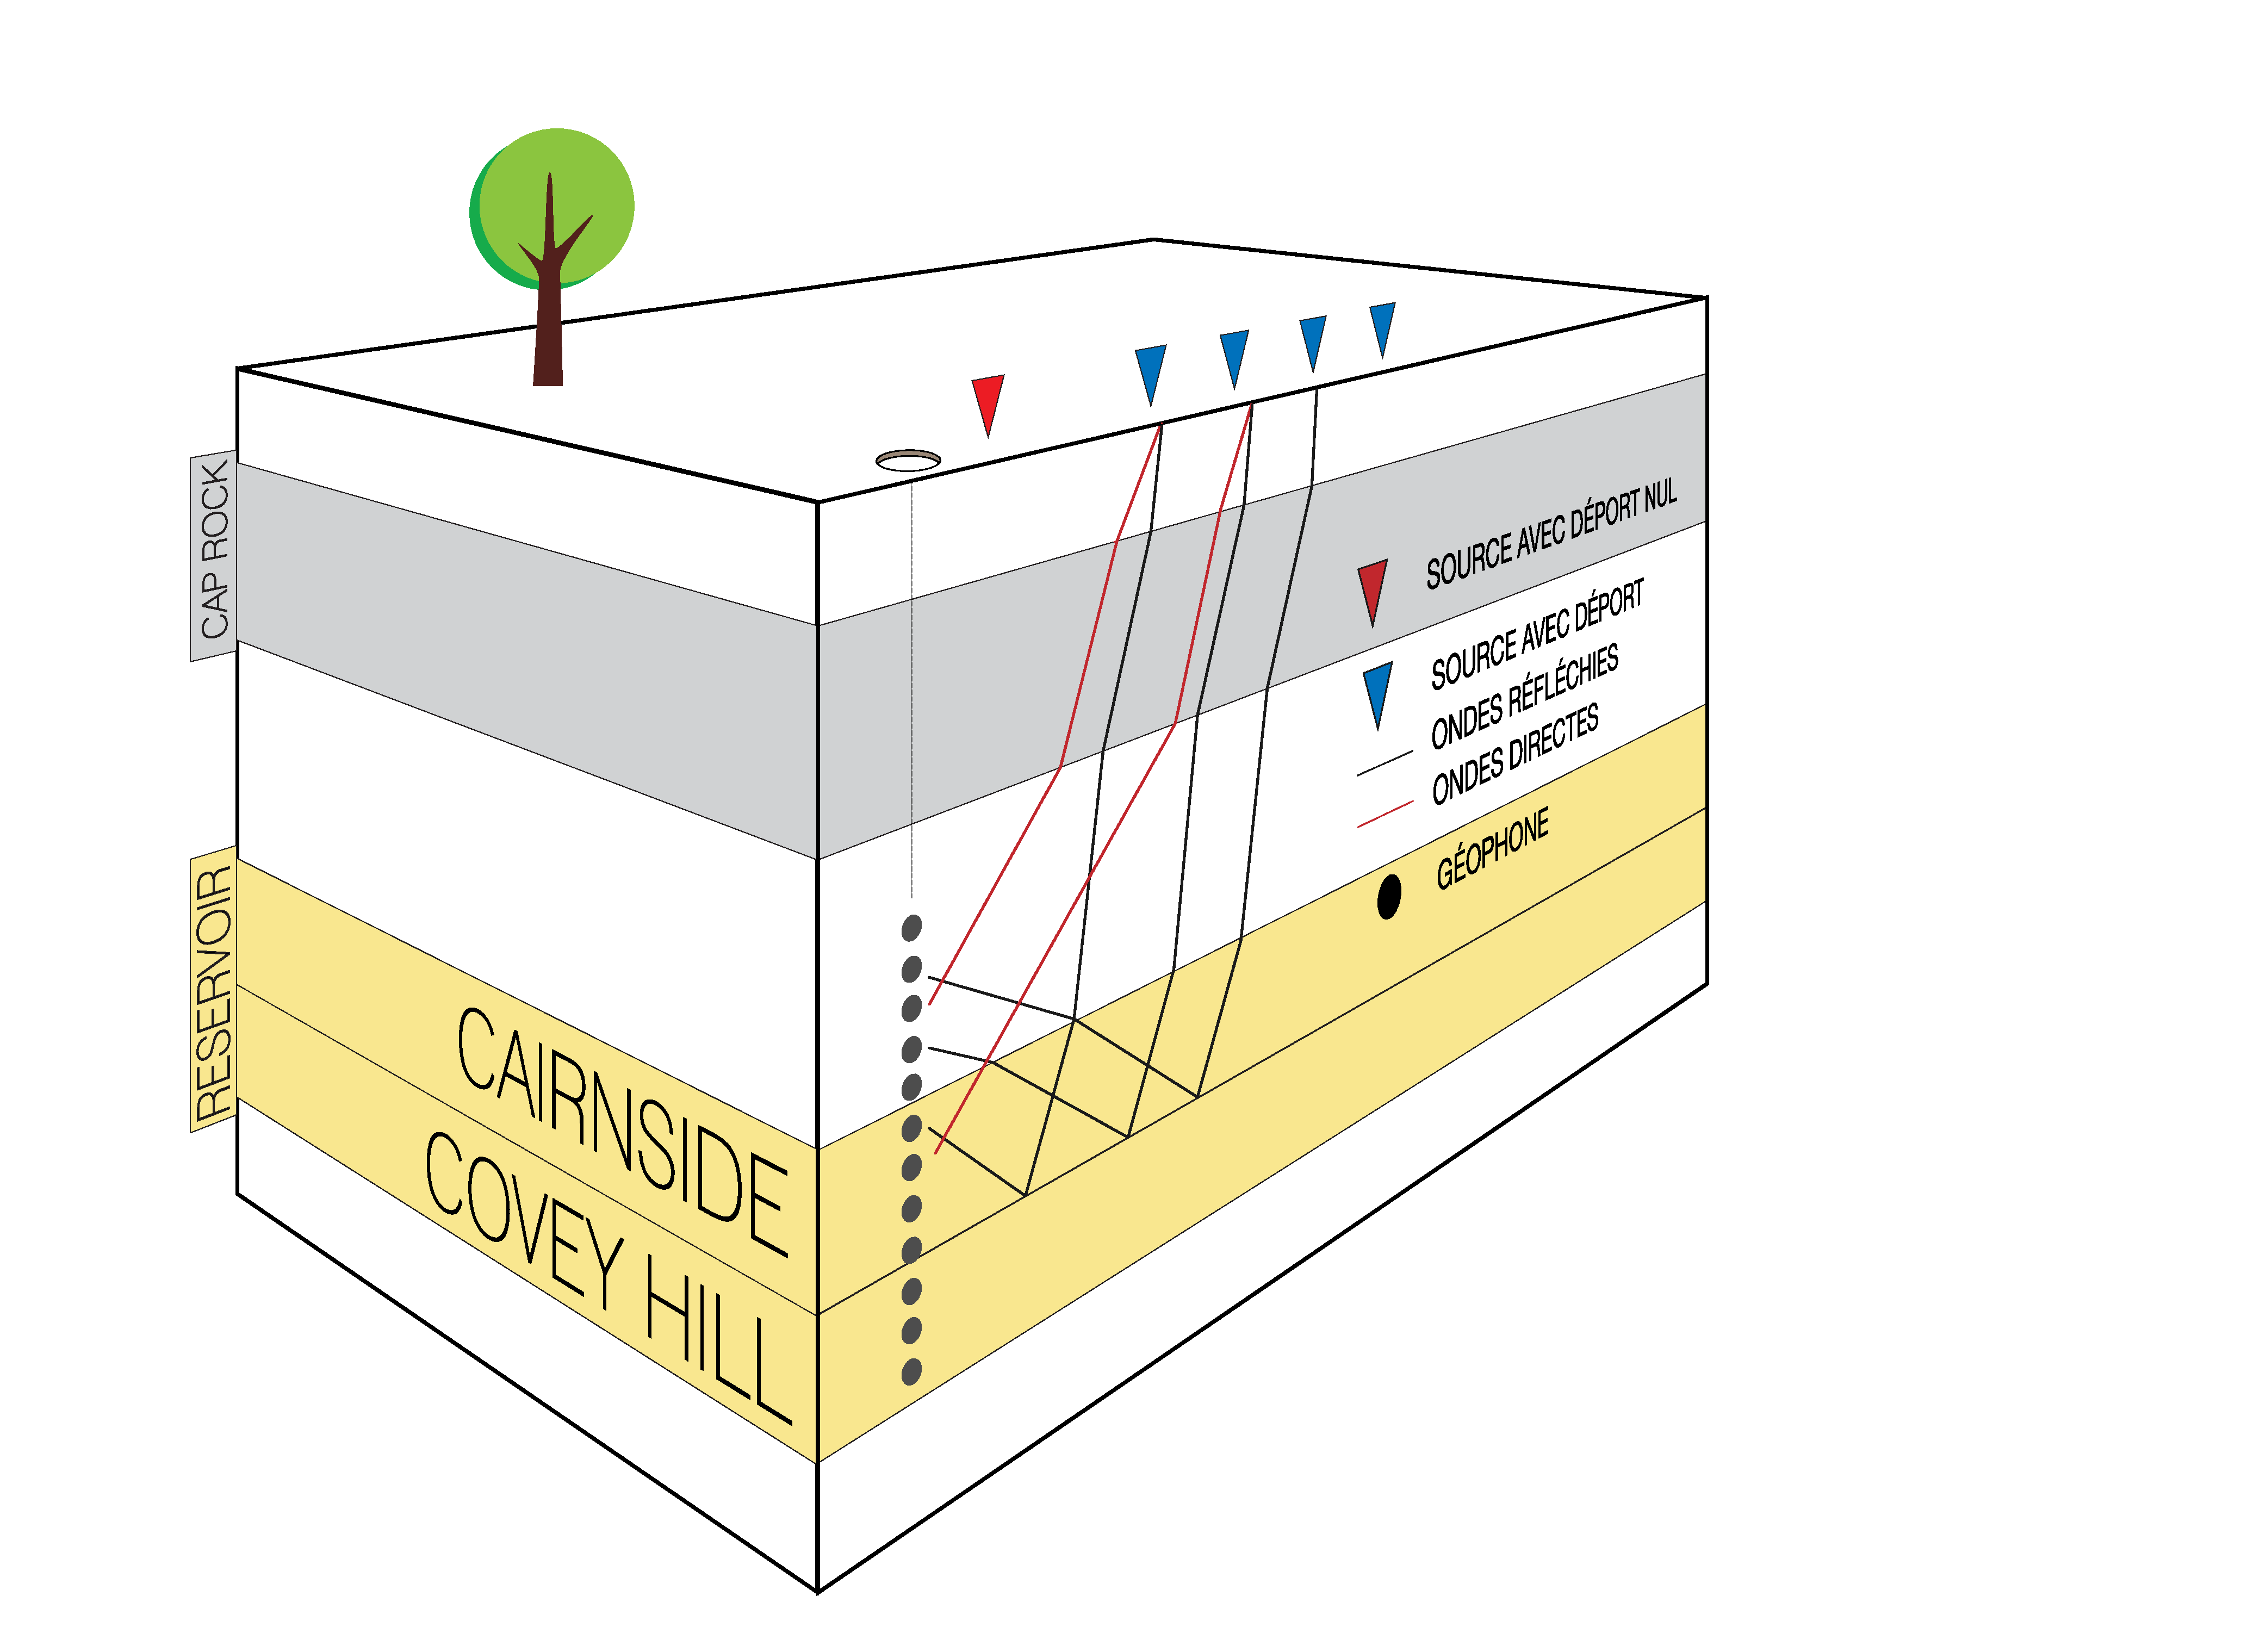
\includegraphics[width=0.8\textwidth]{fig/vsp_3D.pdf}
\caption{Schéma de la géométrie d'acquisition PSV}
\label{fig:vsp_3D}
\end{figure}
La \cref{fig:vsp_3D} montre le schéma d'une acquisition PSV. Une revue exhaustive de cette méthode est présentée dans \citep{Hardage1992,Mari2003}
\subsection{Modèle géologique}
Le modèle géologique utilisé pour la modélisation sismique a été généré à partir de plusieurs forages disponibles dans la zone d'étude \citep{Claprood2012,TranNgoc2014}. À partir des diagraphies, un forage synthétique représentatif pour la région de Bécancour (C'EST LA PREMIÈRE FOIS QUE TU EN PARLES. TU DOIS DÉCRIRE) a été construit pour les valeurs de $V_p$, $V_s$, densité et porosité (voir \cref{fig:well-log} de l'article II à la \cpageref{fig:well-log}). Pour chaque Formation, les distributions de $V_p$, $V_s$, densité et porosité ont été calculées, ainsi que leurs variogrammes verticaux. À partir de ces distributions, un modèle de référence a été généré en utilisant une approche géostatistique par cosimulation séquentielle gaussienne, méthode couramment utilisée pour la modélisation des propriétés géologiques à partir des forages \citep{Deutsch1998,Doyen2007}. Le modèle pour les vitesses des ondes $P$ est présenté à la \cref{fig:mod_ref_vp}.
\begin{figure}[ht]
\centering
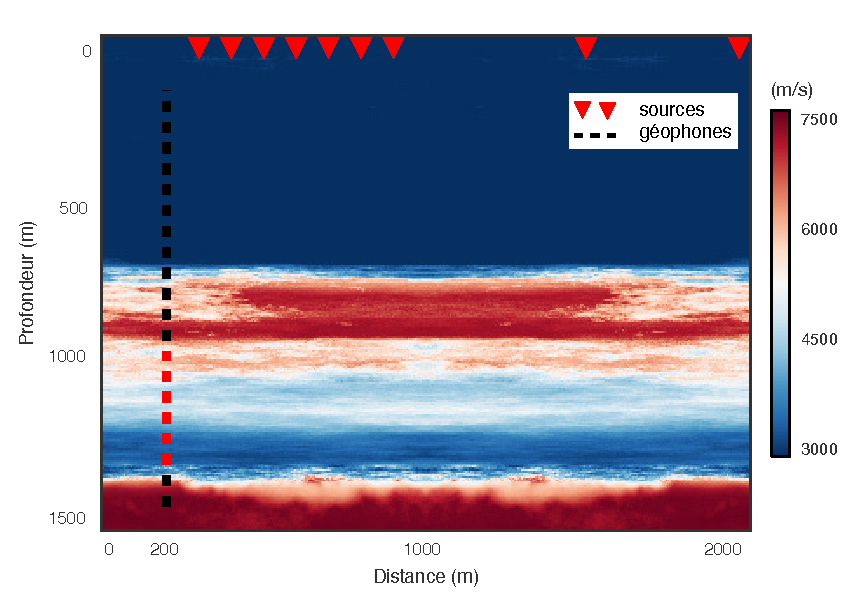
\includegraphics[width=0.8\textwidth]{fig/mod_ref_vp.pdf}
\caption{Modèle de référence pour $V_p$}
\label{fig:mod_ref_vp}
\end{figure}
La taille du modèle, qui fait \SI{2000 x 1500}{\metre} avec un pas de \SI{1 x 1}{\metre} pour un total de \num{3} millions de nœuds est présenté dans la \cref{fig:mod_ref_vp}. Le \cref{tbl:modele} résume les caractéristiques physiques du modèle.
\subsection{Modélisation sismique}
Un code poroviscoélastique basé sur les travaux de \citet{Carcione1995,Carcione1996,Carcione1999} et développé par \citet{Giroux2012} a été utilisé pour générer des sismogrammes synthétiques. L'objectif était d'étudier la performance du PSV pour détecter les changements sur le signal sismique dus à l'injection du \ce{CO2}. Cette formulation prend en compte 12 paramètres, à savoir le module de la roche sèche ($K_{dry}$), le module des minéraux de la roche ($K_s$), le module des fluides interstitiels ($K_{f}$), la porosité ($\phi$), le module de cisaillement de la roche ($G_s$), la densité des minéraux de la roche ($\rho_s$), la densité des fluides interstitiels ($\rho_f$), la tortuosité ($\tau$), la viscosité des fluides ($\eta$), la perméabilité ($\kappa$) et le facteur de qualité ($Q$). Le \cref{tbl:modelpar} de l'article I à la \cpageref{tbl:modelpar}, résume les 12 paramètres du modèle géologique utilisé pour la modélisation sismique. \\
La \cref{fig:mod_ref_vp} montre la géométrie d'acquisition choisie pour la modélisation. Les sources sont placées à la surface du modèle avec un déport allant de \SIrange{100}{2000}{\metre} avec un espacement de \SI{100}{\metre} pour le premier \num{7} déports et de \SIlist{1300;1800} pour les longs déports. Les géophones sont placés dans le puits à \SI{200}{\metre}. Ils s'étendent sur une profondeur de \SIrange{200}{1400}{\metre} avec un espacement de \SI{5}{\metre}. Sur la \cref{fig:mod_ref_vp}, les géophones qui se trouvent dans le réservoir (Formation du Covey Hill et Cairnside) sont mis en évidence en rouge.
L'objectif de la modélisation sismique est de simuler des acquisitions PSV temporelles. Trois suivies ont été simulées: \numlist{5;15;50} ans après injection de \ce{CO2}.
\begin{table}
  \centering
  \caption{Caractéristiques du modèle géologique et géométrie d’acquisition PSV.}
 \begin{tabular}{p{5cm}c}
\toprule
 {Paramètre}  & {Valeur}   \\
\midrule
% Avg. porosity &(\si{\percent})  &  9.75  &  20   \\
% Avg. permeability & (\si{\metre\squared})  & 3.06e-16  & 6.5e-13  \\
Portée en x  & \SI{2000}{\metre}   \\
Portée en z  & \SI{1500}{\metre}   \\
Nœuds  & \num{3} millions   \\
% Injection depth &(\si{\metre}) & \multicolumn{2}{c}{1200-1350 }  \\
% Injection rate &(\si{\tonne\per\metre}) & \multicolumn{2}{c}{45 }  \\
% Injection time &(years) & \multicolumn{2}{c}{15 }  \\
% Migration time &(years) & \multicolumn{2}{c}{35}  \\
% Total storage &(\si{\kilo\tonne}) & \multicolumn{2}{c}{245}\\
Déport des sources  & \SIrange{100}{700}{\metre}    \\
Espacement des sources  & 1\SI{100}{\metre} \\
Coordonnée x des géophones  & \SI{200}{\metre} \\
Coordonnée z des géophones  & \SIrange{200}{1400}{\metre} \\
Espacement des géophones  & \SI{5}{\metre} \\
Traces totales  & 241 \\
\bottomrule
\end{tabular} 
\label{tbl:modele}
\end{table}
\subsubsection{Séquence de traitement}
La séquence de traitement s'inspire du le travail de \citet{Coulombe1996,Zhang2010}. Le \cref{tbl:process} de l'article I à la \cpageref{tbl:process} et la \cref{fig:traitement} résument les étapes du traitement. Il s'agit d'un traitement classique pour les données de PSV, il ne sera pas donc détaillé ici. La séquence de traitement a été appliquée uniquement au déport inférieur à \SI{700}{\metre}; en effet pour les plus grands déports (\SIlist{1300;1800} ), une onde réfractée apparaît à l'interface entre la Formation du Lorraine-Utica et le Groupe Trenton, comme le montre la \cref{fig:refracted} de l'article I à la \cpageref{fig:refracted} et qui empêche la séparation des ondes montantes et descendantes et donc le traitement du PSV. L'analyse des variations des amplitudes avec déports (\emph{Amplitude variation with offset - AVO}) a été donc limitée aux déports inférieurs à \SI{700}{\metre}.
\begin{figure}[!ht]
\centering
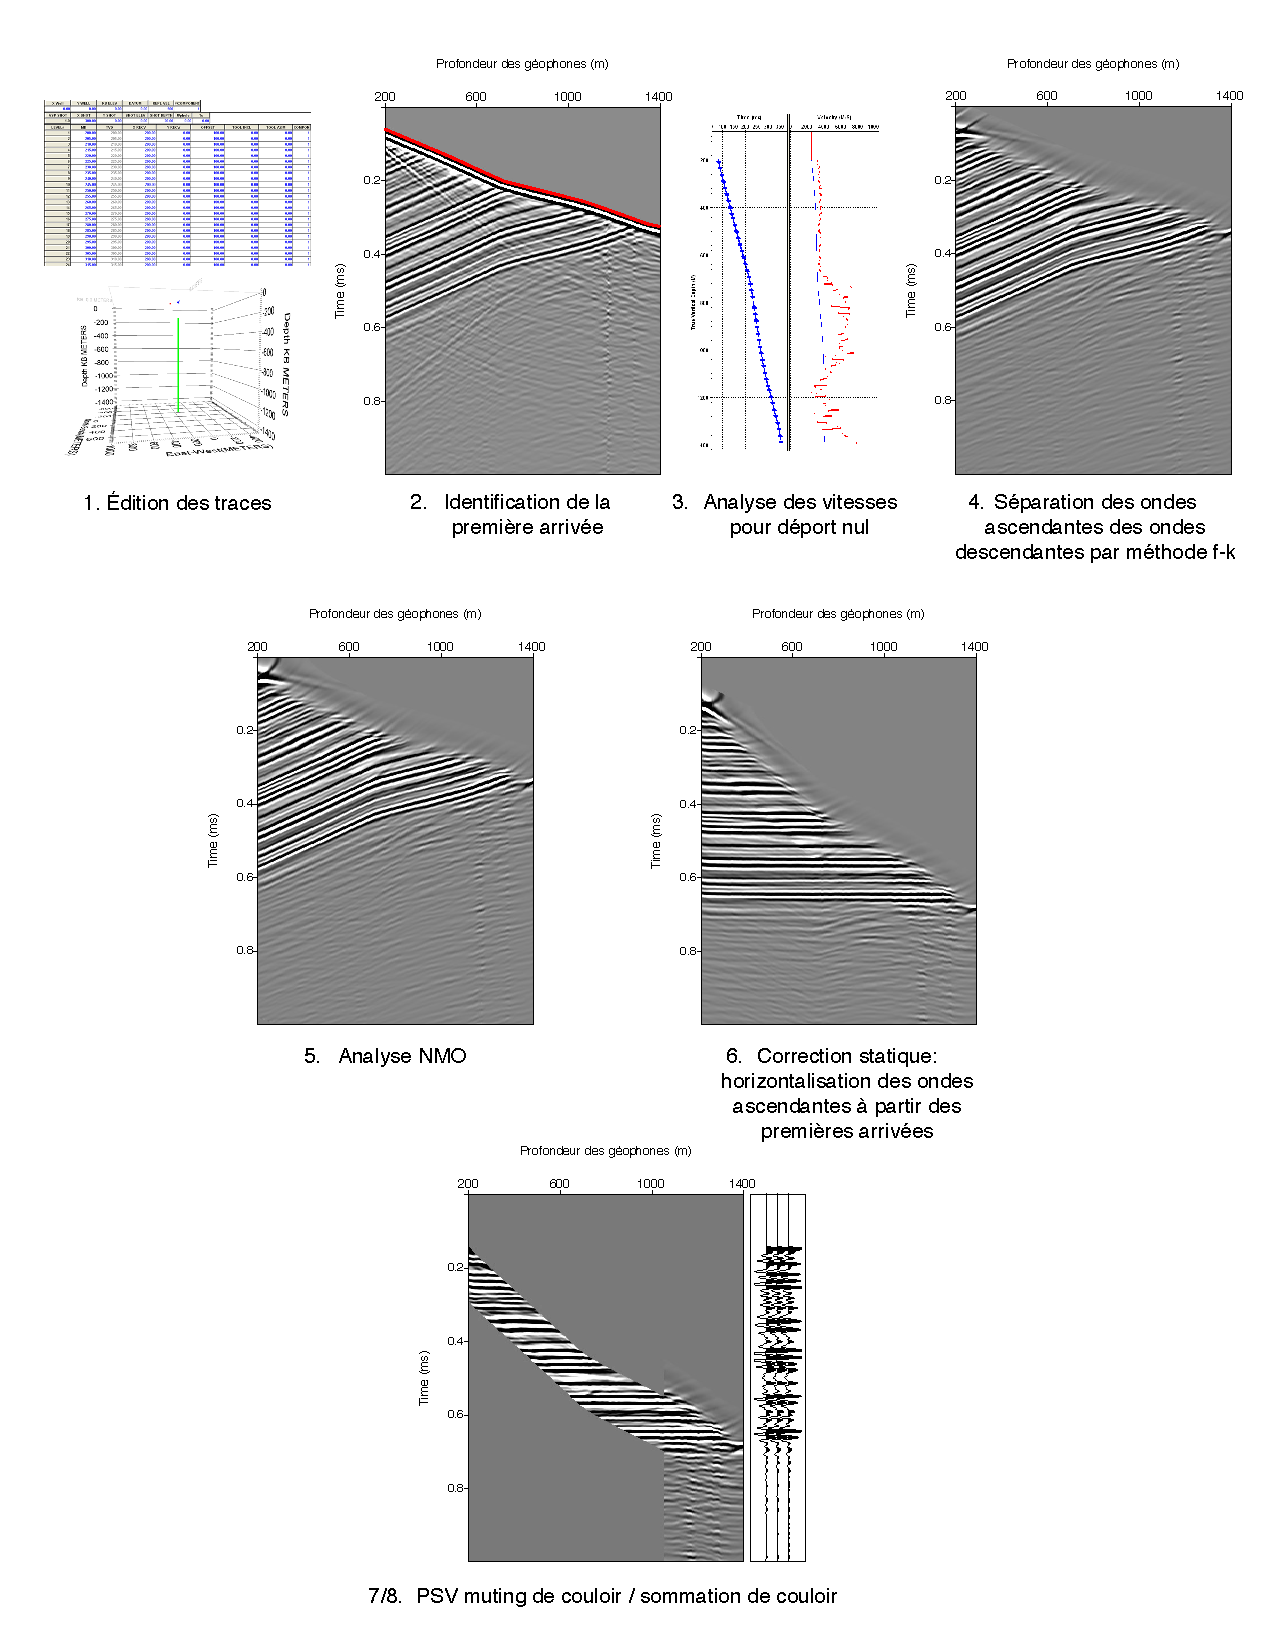
\includegraphics[width=1\textwidth]{fig/traitement.pdf}
\caption{Illustration de la séquence du traitement pour le Profilage Sismique Verticale (PSV).}
\label{fig:traitement}
\end{figure}
\subsection{Modélisation de l'écoulement du \texorpdfstring{\ce{CO2}}{CO2}}
Les approches classiques pour la modélisation de l'injection du \ce{CO2} utilisent 
des méthodes numériques en trois dimensions afin de reproduire avec un degré élevé de précision les effets de l'hétérogénéité et de la dispersion \citep{White1997,Pruess1999,Pruess2004,Schlumberger2007}. Cependant, ces méthodes requirent des efforts informatiques difficiles à reproduire sur des ordinateurs standards.\\
Sous des hypothèses simplificatrices, des modèles qui demandent beaucoup moins d'effort de calcul peuvent être développés. Une de ses hypothèses est d'utiliser des méthodes semi-analytiques, qui ont été de plus en plus développées ces dernières années \citep{Nordbotten2004,Nordbotten2005a,Nordbotten2005,Nordbotten2009}. Cette méthode suppose que l’aquifère soit homogène et horizontal, que il y a une interface définie entre les deux fluides (\ce{CO2} injectée et saumure) et que la géométrie d'injection du \ce{CO2} soit à symétrie radiale \citep{Gasda2009}. Avec ces contraintes, les méthodes analytiques deviennent un outil puissant pour la modélisation de l'injection et de la migration du \ce{CO2}.\\
Une méthode prometteuse pour la modélisation rapide et précise de la séquestration du \ce{CO2} est basée sur l'hypothèse de l'équilibre verticale (VE). Les modèles formulés par VE ont une longue tradition pour la simulation des processus d'écoulement dans les milieux poreux; en hydrologie ils sont connus comme approximation de Dupuit, tandis que dans l'industrie pétrolière ils sont utilisés pour la simulation de l’écoulement multiphase \citep{Martin1958,Coats1967,Martin1968}.\\
Pour modéliser l'écoulement après \numlist{5;15;50} ans du début de l'injection, le modèle à équilibre vertical développé par \citep{Ligaarden2010} et contenu dans MRST - \emph{Matlab Reservoir Simulation Toolbox} \citep{Lie2012} a été utilisé. Dans cette formulation, la saturation moyenne est $s=\frac{h}{H}$ et correspond à la hauteur relative du panache de \ce{CO2}, comme montré sur la \cref{fig:VE}.
\begin{figure}[!ht]
\centering
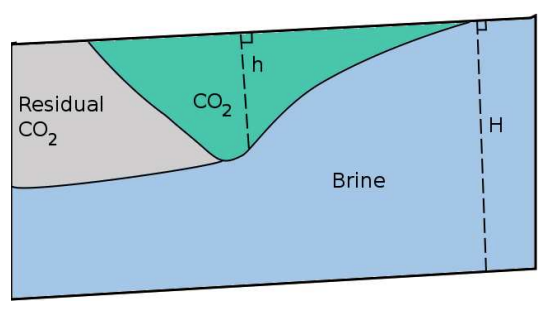
\includegraphics[width=0.7\textwidth]{fig/VE.png}
\caption{Illustration du panache de \ce{CO2} assumé dans les modèles à équilibre vertical (VE), d'après \citet{Ligaarden2010}.}
\label{fig:VE}
\end{figure}
La \cref{fig:res} montre les distributions de porosité et de perméabilité au niveau du réservoir (Formation du Cairnside et du Covey Hill), qui sont utilisés pour simuler l'injection du \ce{CO2}. La pérméabilité est dérivée en utilisant une extension de l'équation de Kozeny-Carman \citep{Kozeny1927,Carman1938}:
\begin{equation}
k = \dfrac{1}{72}\dfrac{\phi^3}{(1-\phi)^2\tau^2}d^2,
\end{equation}
où $d$ est le diamètre des grains qui composent la roche. Pour des grès très compacts, cette valeur est de l'ordre \SI{5e-6}{\metre}. (RÉFÉRENCE) 
\begin{figure}[!ht]
        \centering
        \begin{subfigure}[b]{1\textwidth}
                \caption{Porosité}
                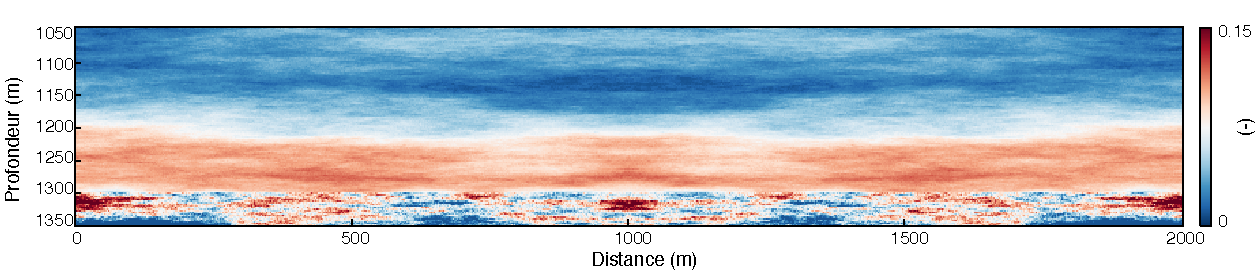
\includegraphics[width=\textwidth]{fig/phi_res.pdf}
                \label{fig:phi_res}
        \end{subfigure}%

        \begin{subfigure}[b]{1\textwidth}
                \caption{Perméabilité}
                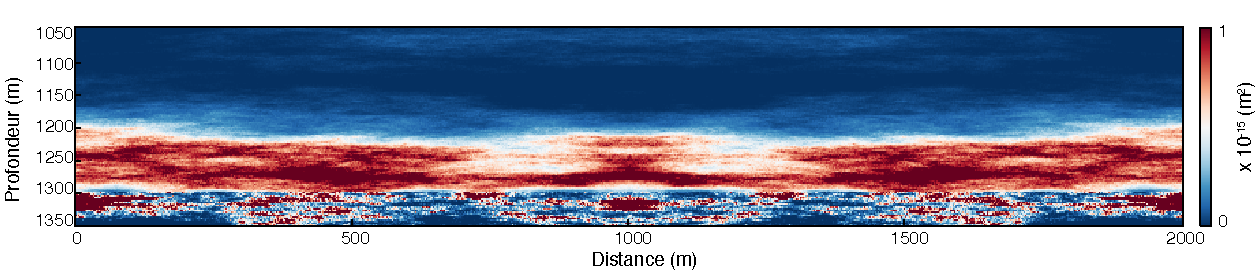
\includegraphics[width=\textwidth]{fig/K_res.pdf}
                \label{fig:K_res}
        \end{subfigure}

        \caption{Distribution de la porosité et de la perméabilité dans le réservoir.}
        \label{fig:res}.
\end{figure}
La simulation d'écoulement se fait dans la formation du Covey Hill (\SIrange{1200}{1350}{\metre}). Le \cref{fig:5r,fig:15r,,fig:50r} montrent l'extension et la saturation du panache de \ce{CO2} après \numlist{5;15;50} ans.\\

Un deuxième scénario, avec une porosité moyenne de \SI{20}{\percent} dans le réservoir (scénario optimal) a été étudié. Les résultats des simulations d'écoulement de \ce{CO2} sont présentés aux \cref{fig:5o,fig:15o,,fig:50o}. Pour ce scénario, l'extension du panache est logiquement plus grande. Les paramètres principaux pour les deux scénarios sont résumés dans le \cref{tbl:co2par} de l'article I à la \cpageref{tbl:co2par}.
% \begin{landscape}
\begin{figure}[!ht]
        \centering
        \begin{subfigure}[b]{.47\textwidth}
                \caption{5 ans après injection \\ Scénario réel }
                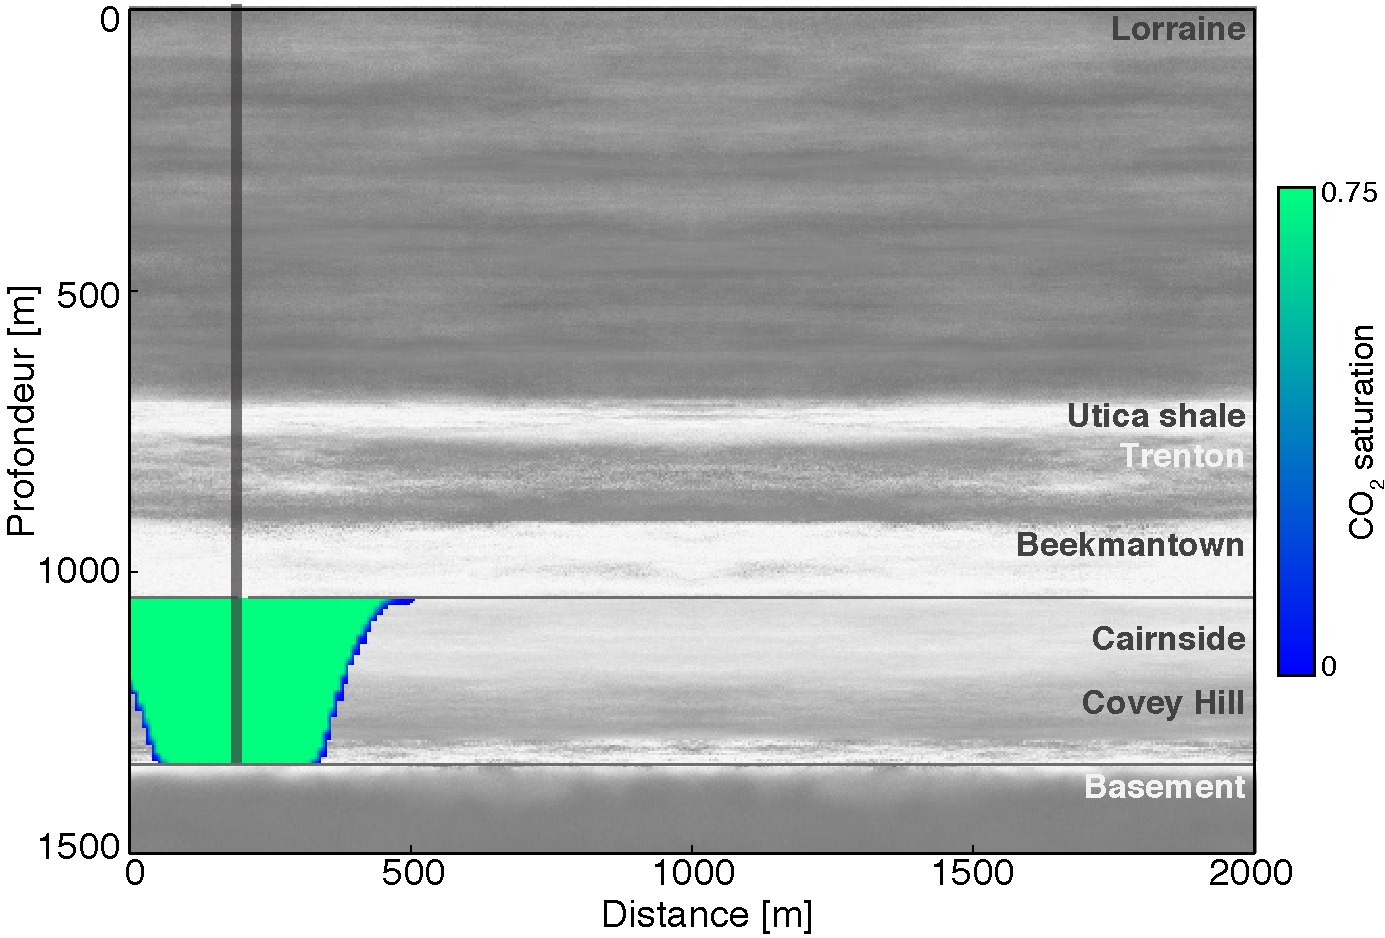
\includegraphics[width=\textwidth]{fig/5r.pdf}
                \label{fig:5r}
        \end{subfigure}
        \qquad
        \begin{subfigure}[b]{.47\textwidth}
                \caption{5 ans après injection \\ Scénario optimal}
                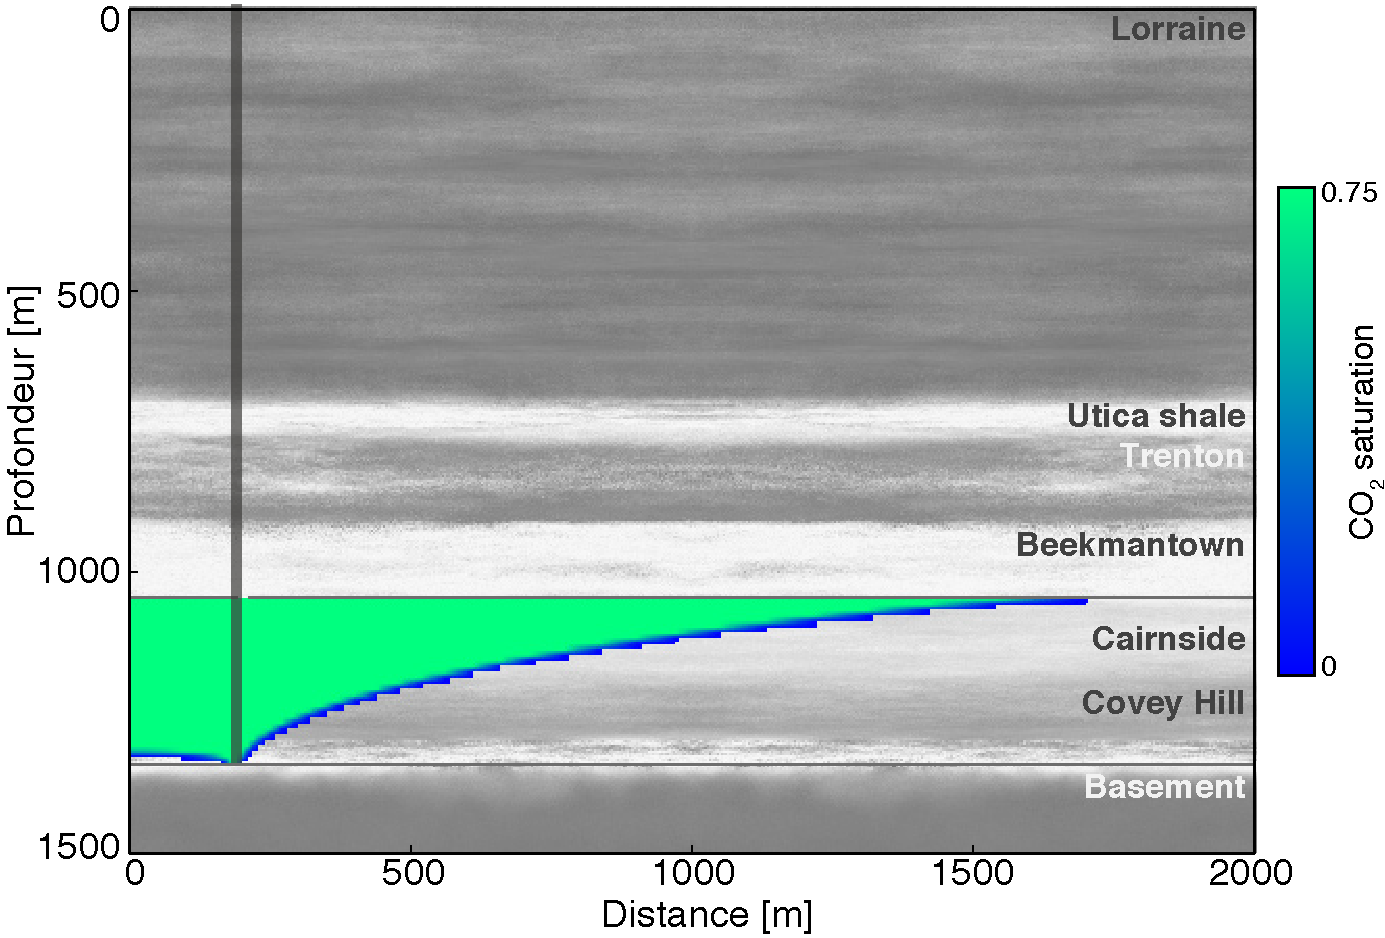
\includegraphics[width=\textwidth]{fig/5o.pdf}
                \label{fig:5o}
        \end{subfigure}
    
        \begin{subfigure}[b]{.47\textwidth}
                \caption{15 ans après injection }
                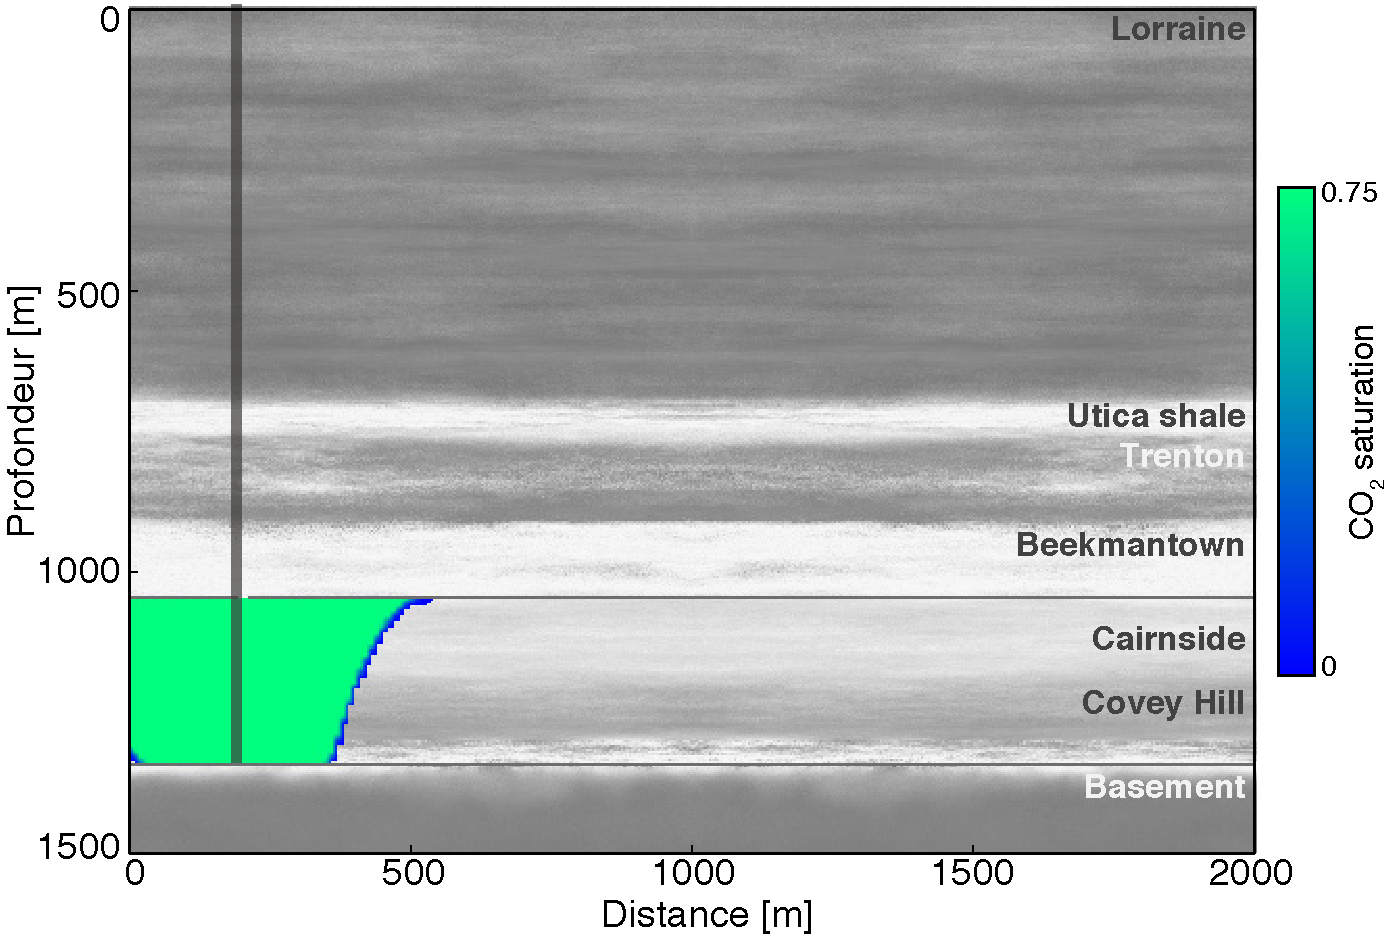
\includegraphics[width=\textwidth]{fig/15r.pdf}
                \label{fig:15r}
        \end{subfigure}
        \qquad
        \begin{subfigure}[b]{.47\textwidth}
                \caption{15 ans après injection  }
                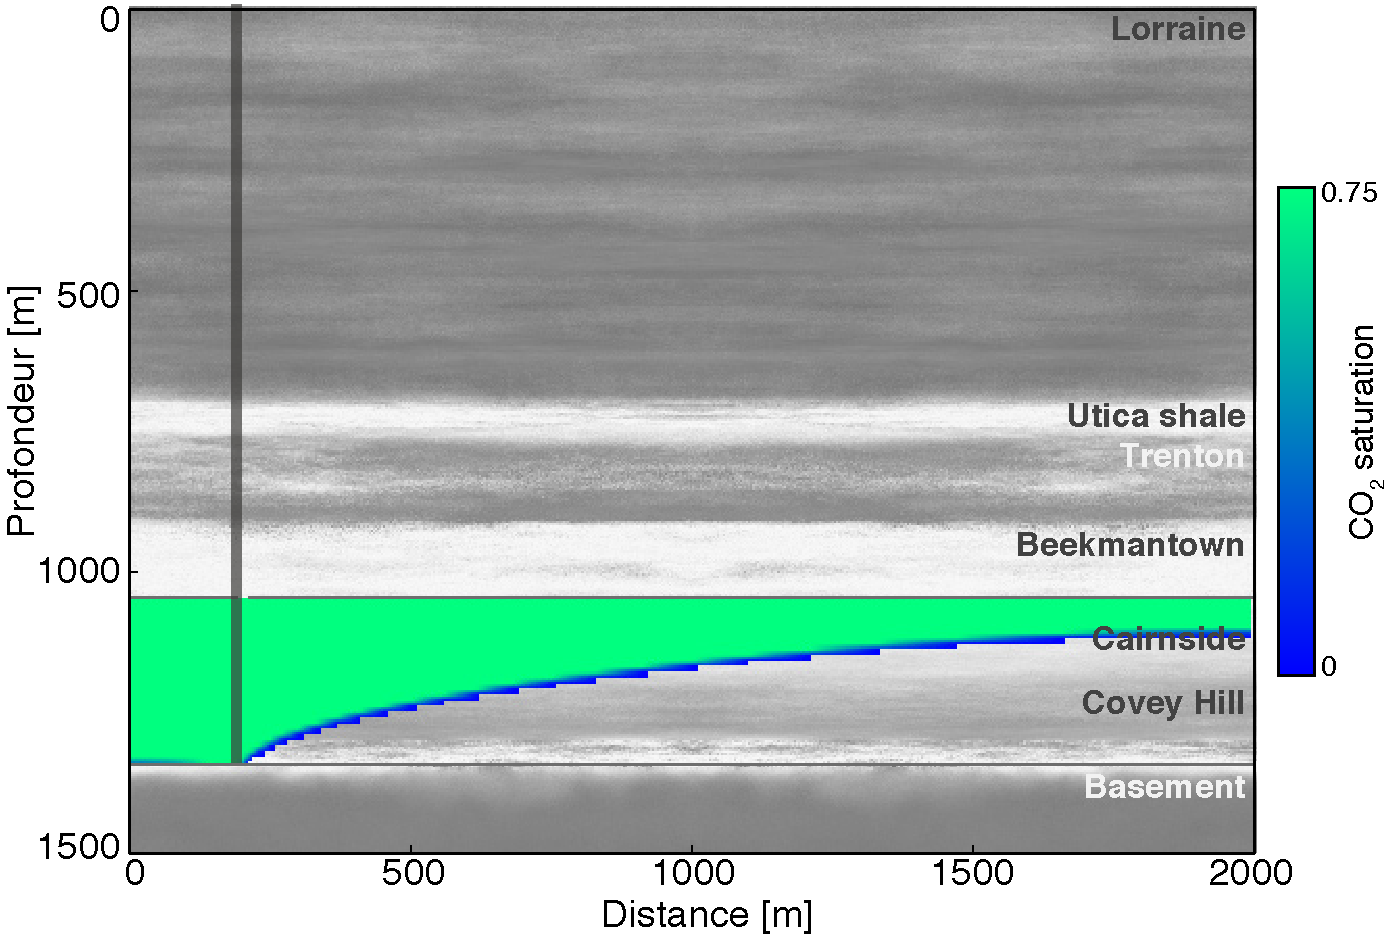
\includegraphics[width=\textwidth]{fig/15o.pdf}
                \label{fig:15o}
        \end{subfigure}

        \begin{subfigure}[b]{.47\textwidth}
                \caption{50 ans après injection }
                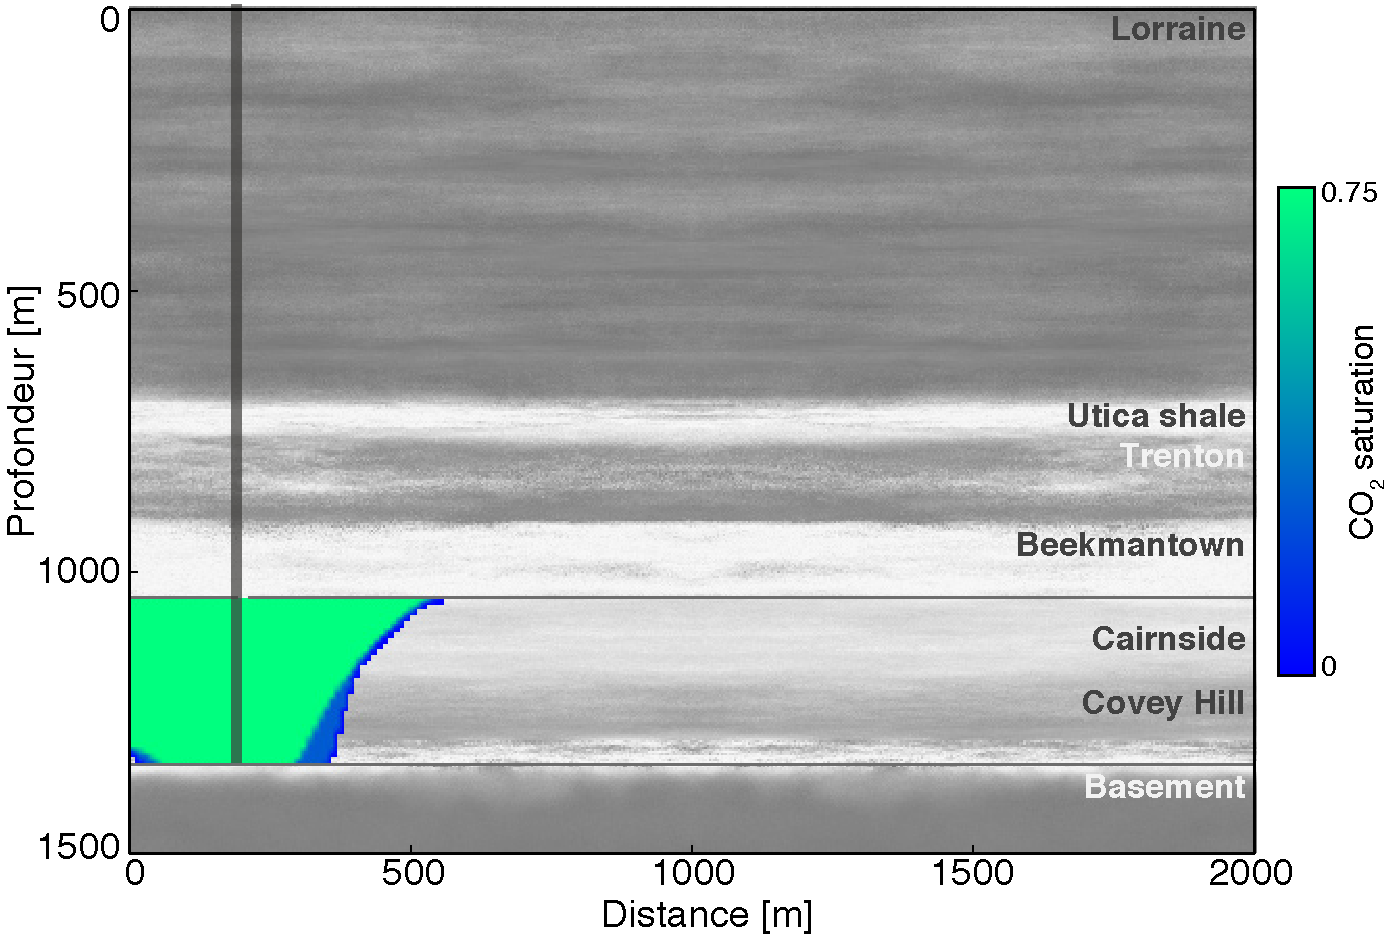
\includegraphics[width=\textwidth]{fig/50r.pdf}
                \label{fig:50r}
        \end{subfigure}
        \qquad
         \begin{subfigure}[b]{.47\textwidth}
                \caption{50 ans après injection}
                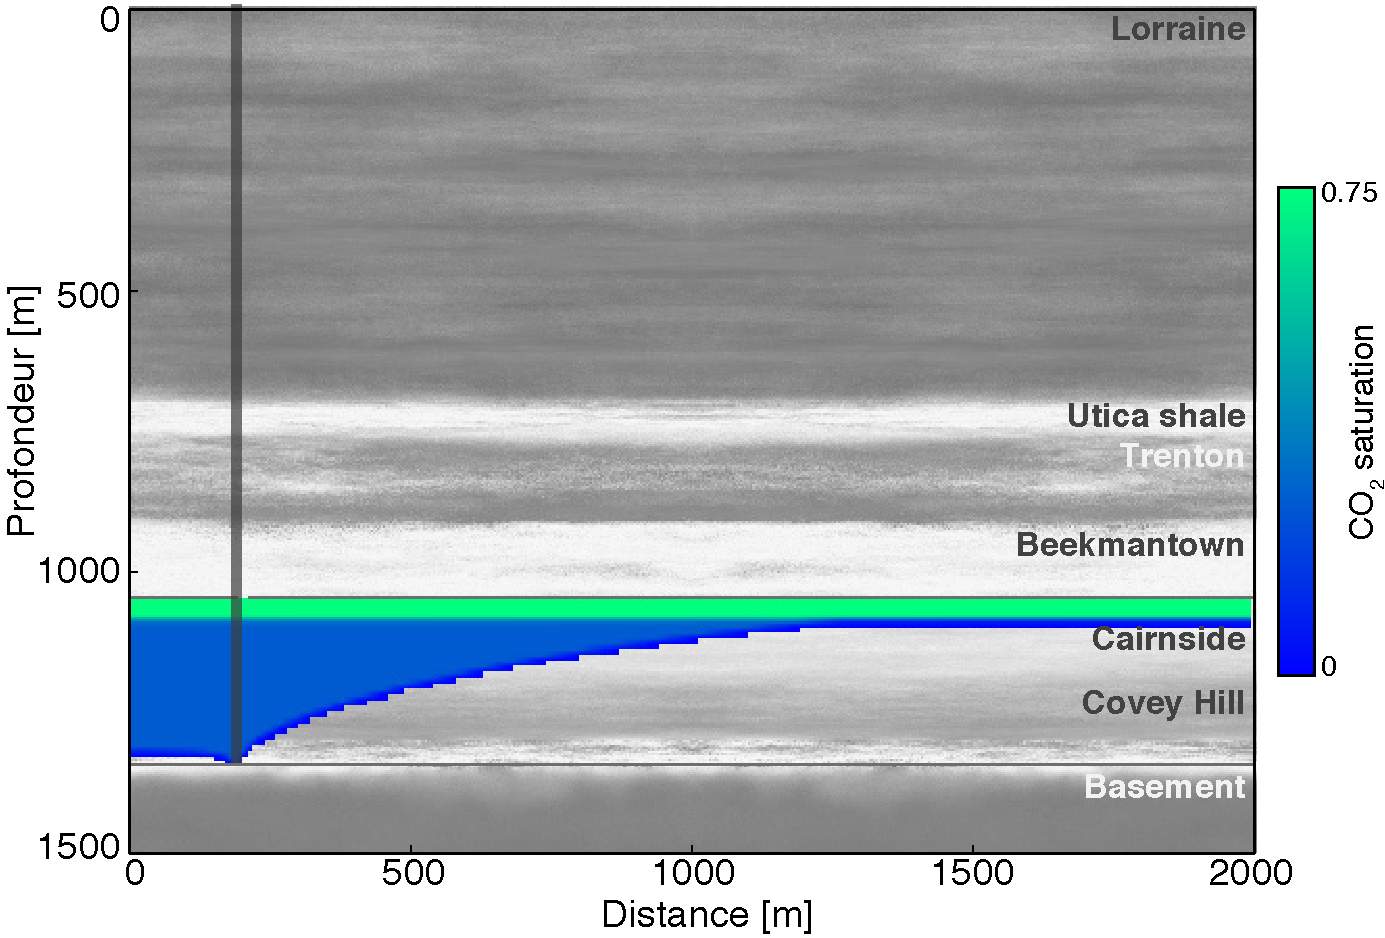
\includegraphics[width=\textwidth]{fig/50o.pdf}
                \label{fig:50o}
        \end{subfigure}
               
        \caption{Saturation du panache du \ce{CO2} en fonction du temps.}
        \label{fig:co2_sat}.
\end{figure}
% \end{landscape}
\subsection{Synthèse des résultats}
Les résultats de la modélisation PSV temporelle pour le scénario optimal et réel sont présentés aux \cref{fig:seismopt,fig:seismbec} de l'article I aux \cpageref{fig:seismopt,fig:seismbec} respectivement. Les deux figures montrent la sommation des traces pour les déports de \SIrange{100}{700}{\metre}. Pour chaque suivi, la modélisation avant injection est représentée par les traces noires.\\
Pour les deux scénarios, un délai dû à l'injection du \ce{CO2} est détecté à partir de \SI{550}{\milli\second}. La sommation des traces donne un résultat généralement très comparable, excepté pour le réflecteur placé à \SI{700}{\milli\second} qui montre une anomalie AVO pour le scénario réel, mais pas pour le scénario optimal. La simulation d'écoulement montre que pour la période de migration du \ce{CO2} (\numrange{15}{50} ans), il y a dissolution partielle du \ce{CO2}. Ce phénomène est plus accentué dans le scénario optimal et il se reflète dans les traces sommées, avec une arrivée légèrement plus précoce pour le réflecteur à \SI{700}{\milli\second} comparé au même réflecteur pour du scénario réel comme le montre la \cref{fig:optvsbec} de l'article I à la \cpageref{fig:optvsbec}.\\
Une comparaison entre le modèle hétérogène proposé et un modèle homogène stratifié classique a été effectuée et les résultats sont présentés aux \cref{fig:stochvsblock_a,fig:stochvsblock_a} de l'article I à la \cpageref{fig:stochvsblock_a} pour un suivi après \num{5} ans du début de l’injection, pour le scénario réel. Cette comparaison permet d’évaluer la différente réponse sismique produite par les deux modèles. Par exemple, le réflecteur à \SI{700}{\milli\second} montre une diminution de l'amplitude avec l'augmentation du déport pour le modèle homogène classique, tandis que pour le modèle hétérogène le même réflecteur montre une augmentation de l'amplitude avec le déport. Ce phénomène est confirmé avec l’analyse de Zœprritz \citep{Aki1980} dans la \cref{fig:zoeppritz} de l'article I à la \cpageref{fig:zoeppritz}.